\documentclass[12pt]{article}
\usepackage[utf8]{inputenc}
\renewcommand{\contentsname}{Cuprins}
\usepackage{latexsym}
\usepackage{url}
\usepackage{hyperref}
\usepackage{lmodern}
\usepackage{graphicx}
\usepackage{mathtools}
\DeclarePairedDelimiter\ceil{\lceil}{\rceil}
\DeclarePairedDelimiter\floor{\lfloor}{\rfloor}
\hypersetup{colorlinks=true}
\graphicspath{ {images/} }

\title{Technical Report}

\author{Grigore Sandi-Gabriel\\
gabigrigore17@gmail.com\\
CEN 2.2 A\\
The University of Craiova\\
}

\date{$6^{th}$ of June 2021}

\usepackage{graphicx}
\usepackage{circuitikz}
\usepackage{tikz}
\usepackage{hyperref}
\usepackage{color}
\usepackage{amsmath}
\usepackage{siunitx}
\usepackage{listings}

\begin{document}
\maketitle
\newpage


\section{Problem Statement}\label{sec_ps}

Suppose two friends live in different cities on a map, such as the Romania map shown
in Figure \ref{fig:Romania}. On every turn, we can simultaneously move each friend to a neighboring city on the map. The amount of time needed to move from city $i$ to neighbor $j$ is equal to the road distance $d(i, j)$ between the cities, but on each turn the friend that arrives first must wait until the other one arrives (and calls the first on his/her cell phone) before the next turn can begin. We want the two friends to meet as quickly as possible.
\begin{itemize}
    \item[a.] Write a detailed formulation for this search problem.
    \item[b.] Identify a search algorithm for this task and explain your choice.
\end{itemize}

\begin{figure}[htp]
    \centering
    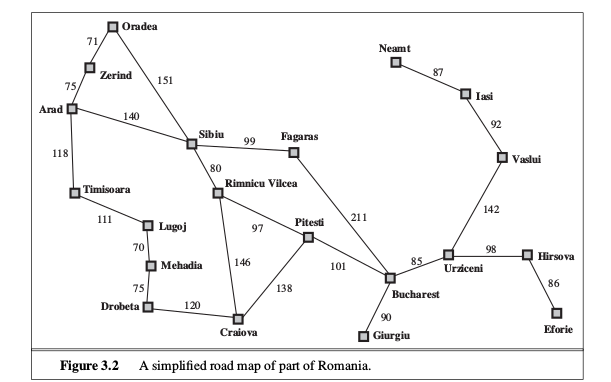
\includegraphics[width=1\textwidth]{Romania.png}
    \caption{Romania Map}
    \label{fig:Romania}
\end{figure}
\newpage
At a first glance, the statement above seems to denote a basic \textbf{"shortest path"} type of problem, but as we'll see shortly, it is more complex than it seems.
\newline
\newline
The goal is simple: \textbf{We have to place both people in the same city in the shortest amount of time possible.} One might think that the shortest path will do the trick but, even though most of the time the shortest path gives us the best time as well, not always will it be the correct answer. We have to pay attention to the fact that the two friends have to wait for each other to arrive in the next city. 
\newline
\newline
Let's take the following example:
\newline
\begin{figure}[htp]
    \centering
    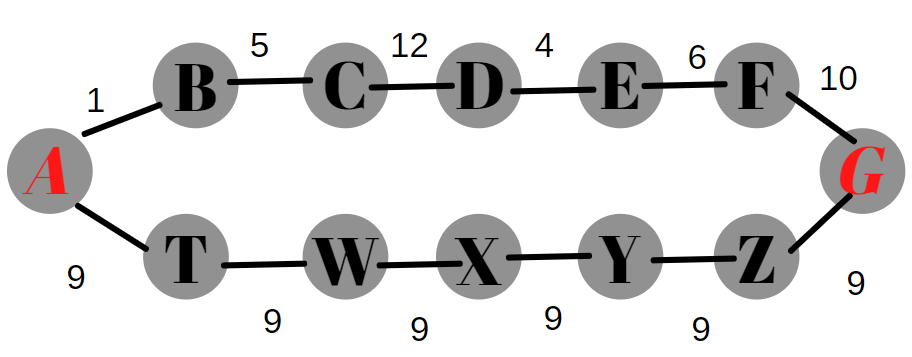
\includegraphics[width=1\textwidth]{route_example.png}
    \caption{Route example}
    \label{fig:Route}
\end{figure}
\newline
In this small example the route above is the shortest and yet the route below takes a smaller amount of time to traverse. This happens because the distribution of the distances is just as important as the length of the path.
Every minute one of the friends has to wait for the other to arrive at their next stop is wasted.
\newline
\textbf{Route above: 38km, 28 minutes}
\newline
\textbf{Route below: 54km, 27 minutes}

\newpage

To solve this problem I used a modified version of \textbf{Yen's algorithm}.
Yen's algorithm computes single-source K-shortest loopless paths for a graph with non-negative edge cost.
\newline
\newline
So as to achieve minimizing the amount of paths I need to evaluate to find the one that has the optimal time, I figured I need to start from the shortest path and work my way up longer paths until a certain \textbf{condition} is met.
\newline
\newline
\textbf{In order to easily understand this condition we have to lay out the following:}
\begin{itemize}
    \item The best case scenario for a path is the one in which neither of the friends has to wait for the other one at any given point. In that scenario the \textbf{path time} will be equal to half of the \textbf{distance of the path}
    \item There is no point in evaluating a path when its best possible time (obtained in the best case scenario) is longer than our current best time
    \item We only evaluate paths in ascending order in terms of distance
\end{itemize}
Considering the above statements, we can now understand why our \textbf{condition} for evaluating the minimum amount of paths possible is to \textbf{stop evaluating paths once the best possible time of the path that is currently being evaluated surpasses our current best time.}
\newline
\newline
In the example above, given than the shortest path takes 28 minutes, there cannot be any better path longer than 56km because even if none of the friends have to wait at all, it will still take longer than 28 minutes for them to meet.
\newline
\newline
\textbf{Language of choice:}
\newline
For this task I came to \textbf{Python} as my language of choice as I find it the most appropriate for working with large data sets and it also lets me focus more on how to solve the problem instead of how to implement the solution. It being a very high level language makes it easier to devise a concise and logical solution that is easily comprehensible by anyone who tries to read it.
\newpage

\section{Pseudocode of Algorithms}\label{sec_ps}
The following pseudocode represents the heart of the whole project, Yen's algorithm for single-source K-shortest loopless paths for a graphwith non-negative edge cost. The only modifications I made are the following: I needed an extra array to store the total distance of every path and an extra array to store the total time of every path.
\newline
\begin{lstlisting}[language=C]
function YenKSP(Graph, source, sink, K):
    // Determine the shortest path from the source to the sink.
    A[0] = Dijkstra(Graph, source, sink);
    // Initialize the set to store the potential kth shortest path.
    A_len = sum(edges)
    A_time = sum(max(first_edge, last_edge))
    
    B = [];
    
    for k from 1 to K:
        // The spur node ranges from the first node to 
        //the next to last node in the previous k-shortest path.
        for i from 0 to size(A[k − 1]) − 2:
            
            // Spur node is retrieved from the previous 
            //k-shortest path, k − 1.
            spurNode = A[k-1].node(i);
            // The sequence of nodes from the source to 
            //the spur node of the previous k-shortest path.
            rootPath = A[k-1].nodes(0, i);
            
            for each path p in A:
                if rootPath == p.nodes(0, i):
                    // Remove the links that are part of 
                    //the previous shortest paths which 
                    //share the same root path.
                    
                    //remove p.edge(i,i + 1) from Graph;
            
            for each node rootPathNode in rootPath except spurNode:
                remove rootPathNode from Graph;
            
            // Calculate the spur path from the spur 
            //node to the sink.
            // Consider also checking if any spurPath found
            spurPath = Dijkstra(Graph, spurNode, sink);
            
            // Entire path is made up of the root path 
            //and spur path.
            totalPath = rootPath + spurPath;
            // Add the potential k-shortest path to the heap.
            if (totalPath not in B):
                B.append(totalPath);
            
            // Add back the edges 
            /and nodes that were removed from the graph.
            restore edges to Graph;
            restore nodes in rootPath to Graph;
                    
        if B is empty:
            // This handles the case of there being no 
            //spur paths, or no spur paths left.
            // This could happen if the spur paths have 
            //already been exhausted (added to A), 
            // or there are no spur paths at all - such 
            //as when both the source and sink vertices 
            // lie along a "dead end".
            break;
        // Sort the potential k-shortest paths by cost.
        B_len = sum(edges) for every path in B
        B.sort();
        for path in B
            B_time.append(sum(max(first_edge, last_edge))
        // Add the lowest cost path becomes the k-shortest path.
        A[k] = B[0];
        A_time.append(B_time)
        A_len.append(B_len)
        // In fact we should rather use shift since we 
        //are removing the first element
        B.pop();
    
    return A, A_len, A_time;

\end{lstlisting}

\section{Application Outline}\label{sec_ps}
\subsection{The high level architectural overview of the application}
My application intends on abstracting the logic behind the scenes by providing an easy-to-use interface that is used in the \textbf{main.py} module. This interface only demands a data source in the form of a \textbf{json} file and the cities whose optimal path you need to find.
\newline\newline
On the other hand, the real magic happens behind the scenes. Over there, the data source is read and its contents are interpreted in order to build a graph that represents our map. After that we find the shortest path (by distance) via Dijkstra's algorithm. Following this we inspect the smallest amount possible of the next shortest paths via my modified version of Yen's algorithm in order to make sure we find the most optimal (time-wise) path in the map. When all of this is over, one of the functions interprets the resulting data and outputs the most relevant information to the console.

\subsection{The specification of the input data format}
The input data takes the form of a \textbf{json file} and its format is the following (based on the example used above):
\begin{lstlisting}[language=C]
  "small_sample": {
    "1": {
      "source": "A","target": "B","weight": 1
    },
    "2": {
      "source": "B","target": "C","weight": 5
    },
    "3": {
      "source": "C","target": "D","weight": 12
    },
    "4": {
      "source": "D","target": "E","weight": 4
    },
    "5": {
      "source": "E","target": "F","weight": 6
    },
    "6": {
      "source": "F","target": "G","weight": 10
    },
    "7": {
      "source": "A","target": "T","weight": 9
    },
    "8": {
      "source": "T","target": "W","weight": 9
    },
    "9": {
      "source": "W","target": "X","weight": 9
    },
    "10": {
      "source": "X","target": "Y","weight": 9
    },
    "11": {
      "source": "Y","target": "Z","weight": 9
    },
    "12": {
      "source": "Z","target": "G","weight": 9
    }
  },

\end{lstlisting}
\newpage
\subsection{The specification of the output data format}
The output data is presented in the console and has 
the following format (based on the example used above):
\begin{lstlisting}[language=C]
The optimal route between A and G will 
take 27 minutes and spans over 54 kilometers
The friends will meet in X
The path is the following:
A T W X Y Z G 
\end{lstlisting}
\subsection{The list of all the modules in the application and their description}
The application is composed of the following modules:
\begin{itemize}
    \item \textbf{route\_generator.py}
    \newline
    This is the brain of the application as it contains the main algorithm. It contains only one class that can create map-like objects (based on graphs) that can be interacted with.
    \item \textbf{main.py}
    \newline
    This is the entry point into the application. This is where the actual maps are created and interacted with. This is the module that is supposed to be executed and played with in order to test different scenarios. Here is where I left examples ranging from small (10 cities) to very large (5000 cities).
    \item \textbf{data\_generator.py}
    \newline
    This is the module that auto-generates test data sets based on multiple adjustable parameters. Over 90\% of the data sets used for experimentation in \textbf{main.py} were produced using this generator.
\end{itemize}

Other important files:
\begin{itemize}
    \item \textbf{samples.json}
    \newline
    This is the file that contains the \textbf{DEMO} data sets that can be used to quickly evaluate the efficiency of the algorithm. They have been thoroughly tested.
    \item \textbf{requirements.txt}
    \newline
    This is the file that states which python package must be downloaded for the application to work (networkx).
    \item \textbf{cities.txt}
    \newline
    This is a file that contains 10000 random cities extracted from an online data set. It is used for generating the data sets we need.
    \item \textbf{generated\_data\_.... .json}
    \newline
    These are the data sets generated by my generator.
\end{itemize}
\subsection{The list of all the functions in the application, grouped by modules}
\textbf{route\_generator.py:}
\begin{itemize}
    \item \textbf{k\_shortest\_paths(self, source, target, k=1)}
    \newline
    This function represents the main algorithm (my modified version of \textbf{Yen's Algorithm}. It expects a the starting node, the target node and the amount of short paths you need. It returns three ordered lists containing the paths, their lengths and the time it takes to traverse them.
    \item \textbf{load\_data(self, json\_file, data\_set)}
    \newline
    This function loads the data you provide into the map-like object. It expects the name of the file and the name of the section within it that you want to load in. This function does not return anything
    \item \textbf{optimal\_route(self, source, target, k=3)}
    \newline
    This function analyzes the data provided by the first function in order to find the optimal path. In order to evaluate as few paths as possible, it starts by only evaluating 3 and if those are not enough it recursively calls a version of itself that evaluates one more path than before. It expects the parameters needed by the first function and returns the parameters of the optimal route (the time, the distance and the route).
    \item \textbf{print\_optimal\_route(self, source, target)}
    \newline
    This function is the one we interact with as it only demands the two cities and it provides the result of the search in a readable, easy to understand way. It does not return anything.
\end{itemize}
\textbf{data\_generator.py:}
\begin{itemize}
    \item \textbf{\_\_init\_\_(self, number\_of\_nodes=25, min\_weight=50, max\_weight=300, min\_edges=25, max\_edges=300)}
    \newline
    This is the constructor of the generator. It lets you customize every parameter of the auto-generated data set. None of the parameters are mandatory as they have default values. It also performs check for invalid parameters.
    \item \textbf{json\_dump\_random\_data(self, json\_file)}
    \newline
    This function generates the random data and it dumps it inside the json file that you provide. It doesn't return anything.
    
\end{itemize}
\textbf{main.py has no functions}
\section{Experimental Data:}
\subsection{Introduction:}
In order to test my application I had to build a data generator that could provide me with an infinite amount of data sets ranging from small to very large.
\newline\newline
\textbf{How it works:}
\newline
The generator has its default values for the dimensions of the data set but everything can be modified by the user: the number of cities (we'll call this parameter \textbf{n}); the range in which the distance between two cities can be generated; the range in which the generator will choose a random number of roads to be built between cities (we'll call this parameter \textbf{e}).
\newline\newline
When the parameters are set (by the user or to default), the algorithm starts the generation. From the file \textbf{cities.txt}, the algorithm randomly chooses \textbf{n} cities from the total of 10000. After that we randomly choose a pair of two cities, we check if this pair has ever been previously selected, and if not, we assign it an edge with a random weight within the desired interval. We repeat this process until we have an \textbf{e} amount of unique edges.\newline
\newline
When this process is over, we dump the resulting \textbf{python dictionary} into a \textbf{json} file with the name specified by the user.
\newpage
\subsection{Experiments and results:}
In this subsection I am going to present the results generated by experimenting with 10 randomly generated data sets raging in size from small to very large:
\newline
\newline
\textbf{SMALL:}
\newline
The results from testing generated\_data\_1\_small.json:
\newline
Nodes: 10
\newline
Edges: 14
\newline
Execution time: 0.006s
\begin{figure}[htp]
    \centering
    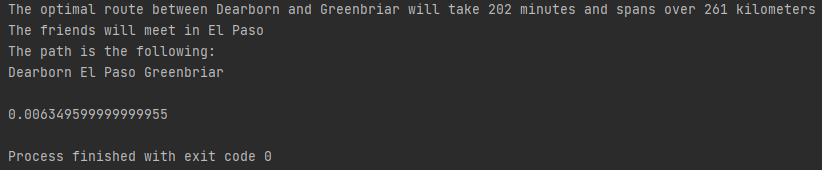
\includegraphics[width=1\textwidth]{small1.png}
\end{figure}
\newline
The results from testing generated\_data\_2\_small.json:
\newline
Nodes: 15
\newline
Edges: 23
\newline
Execution time: 0.007s
\begin{figure}[htp]
    \centering
    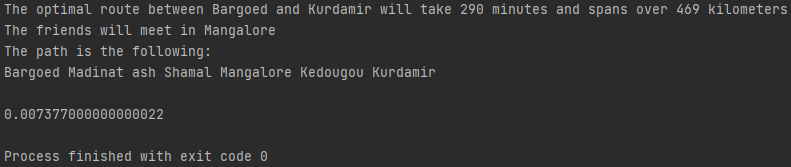
\includegraphics[width=1\textwidth]{small2.png}
\end{figure}
\newpage
The results from testing generated\_data\_3\_small.json:
\newline
Nodes: 20
\newline
Edges: 31
\newline
Execution time: 0.006s
\begin{figure}[htp]
    \centering
    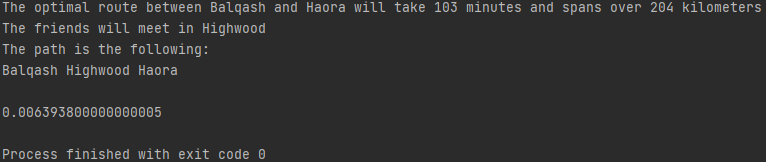
\includegraphics[width=1\textwidth]{small3.png}
\end{figure}
\newline
\newline
\textbf{MEDIUM:}
\newline
The results from testing generated\_data\_4\_medium.json:
\newline
Nodes: 40
\newline
Edges: 108
\newline
Execution time: 0.011s
\begin{figure}[htp]
    \centering
    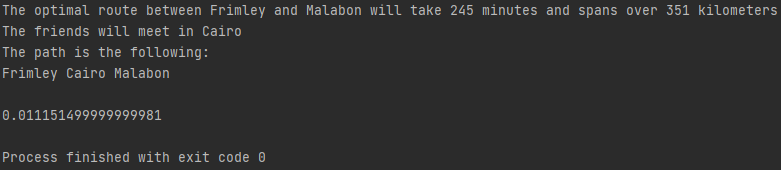
\includegraphics[width=1\textwidth]{medium1.png}
\end{figure}
\newline
The results from testing generated\_data\_5\_medium.json:
\newline
Nodes: 60
\newline
Edges: 140
\newline
Execution time: 0.008s
\begin{figure}[htp]
    \centering
    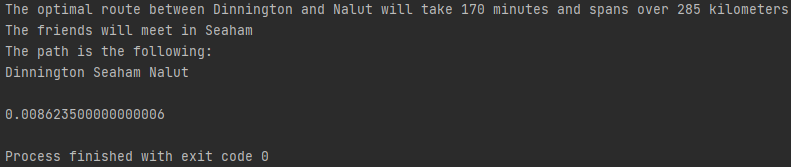
\includegraphics[width=1\textwidth]{medium2.png}
\end{figure}
\newpage
\newline
The results from testing generated\_data\_6\_medium.json:
\newline
Nodes: 80
\newline
Edges: 173
\newline
Execution time: 0.006s
\begin{figure}[htp]
    \centering
    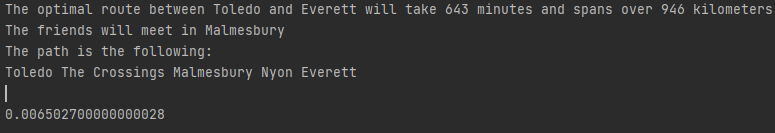
\includegraphics[width=1\textwidth]{medium3.png}
\end{figure}
\newline
\newline
\textbf{LARGE:}
\newline
The results from testing generated\_data\_7\_large.json:
\newline
Nodes: 150
\newline
Edges: 316
\newline
Execution time: 0.008s
\begin{figure}[htp]
    \centering
    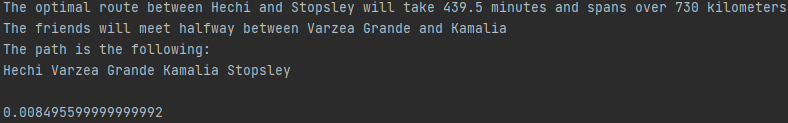
\includegraphics[width=1\textwidth]{large1.png}
\end{figure}
\newline
The results from testing generated\_data\_8\_large.json:
\newline
Nodes: 200
\newline
Edges: 485
\newline
Execution time: 0.007s
\begin{figure}[htp]
    \centering
    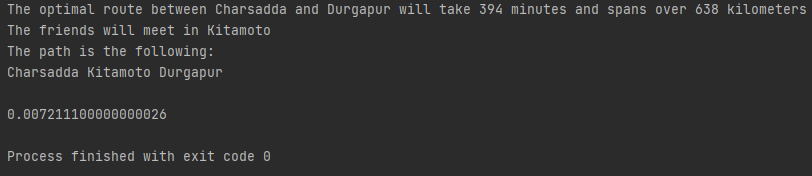
\includegraphics[width=1\textwidth]{large2.png}
\end{figure}
\newline
The results from testing generated\_data\_9\_large.json:
\newline
Nodes: 250
\newline
Edges: 427
\newline
Execution time: 0.006s
\begin{figure}[htp]
    \centering
    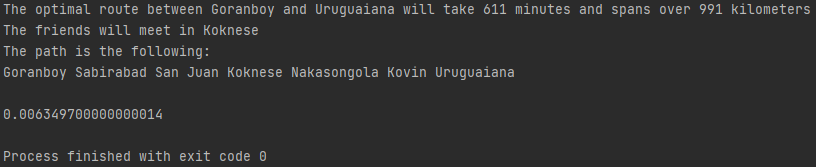
\includegraphics[width=1\textwidth]{large3.png}
\end{figure}
\newline
The results from testing generated\_data\_10\_very\_large.json:
\newline
Nodes: 5000
\newline
Edges: 10177
\newline
Execution time: 0.006s
\begin{figure}[htp]
    \centering
    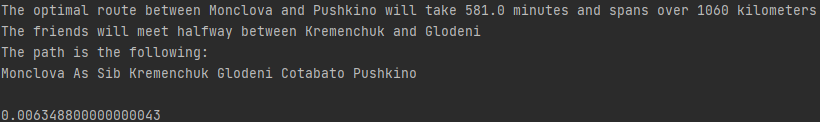
\includegraphics[width=1\textwidth]{very_large.png}
\end{figure}
\newline\newline
\textbf{All of these tests are available in main.py and can be evaluated by the reader. Execution time may vary.}
\section{Conclusions:}
As to conclude this assignment I have to mention that I really enjoyed the process of building this project from the ground up. The hardest part by far was to translate my ideas into python code because even though I had no problem understanding how the problem worked, making the computer understand how the problem works is never as easy.\newline
My favorite part of the whole project was the research. During the research I got to better my understanding of graph theory as well as discovering a lot of different search algorithms by reading dissertations, articles and online forum posts. I also got to interact with people over the internet who've had similar problems in the past. That is how I stumbled upon Yen's Algorithm, the heart of my application. I don't think I will extend this assignment further but I will for sure use the knowledge I needed to aquire to solve it in the future.
\section{References:}

    \caption{
    \textbf{1.} Yen's Algorithm \textbf{https://en.wikipedia.org/wiki/Yen\%27s\_algorithm}\\\\
    \textbf{2.} Dijkstra's algorithm with path \textbf{https://www.geeksforgeeks.org/printing-paths-dijkstras-shortest-path-algorithm/}\\\\
    \textbf{3.} Python interpretation of Yen \textbf{https://github.com/beegeesquare/k-shortest-path}\\\\
    \textbf{4.} Networkx \textbf{https://networkx.org/}\\\\
    }
\end{document}
